%Version 3.1 December 2024
% See section 11 of the User Manual for version history
%
%%%%%%%%%%%%%%%%%%%%%%%%%%%%%%%%%%%%%%%%%%%%%%%%%%%%%%%%%%%%%%%%%%%%%%
%%                                                                 %%
%% Please do not use \input{...} to include other tex files.       %%
%% Submit your LaTeX manuscript as one .tex document.              %%
%%                                                                 %%
%% All additional figures and files should be attached             %%
%% separately and not embedded in the \TeX\ document itself.       %%
%%                                                                 %%
%%%%%%%%%%%%%%%%%%%%%%%%%%%%%%%%%%%%%%%%%%%%%%%%%%%%%%%%%%%%%%%%%%%%%

%\documentclass[referee,sn-basic]{sn-jnl}% referee option is meant for double line spacing

%%=======================================================%%
%% to print line numbers in the margin use lineno option %%
%%=======================================================%%

%%\documentclass[lineno,pdflatex,sn-basic]{sn-jnl}% Basic Springer Nature Reference Style/Chemistry Reference Style

%%=========================================================================================%%
%% the documentclass is set to pdflatex as default. You can delete it if not appropriate.  %%
%%=========================================================================================%%

%%\documentclass[sn-basic]{sn-jnl}% Basic Springer Nature Reference Style/Chemistry Reference Style

%%Note: the following reference styles support Namedate and Numbered referencing. By default the style follows the most common style. To switch between the options you can add or remove Numbered in the optional parenthesis. 
%%The option is available for: sn-basic.bst, sn-chicago.bst%  
 
%%\documentclass[pdflatex,sn-nature]{sn-jnl}% Style for submissions to Nature Portfolio journals
%%\documentclass[pdflatex,sn-basic]{sn-jnl}% Basic Springer Nature Reference Style/Chemistry Reference Style
%% \documentclass[pdflatex,sn-mathphys-num]{sn-jnl}% Math and Physical Sciences Numbered Reference Style
%%\documentclass[pdflatex,sn-mathphys-ay]{sn-jnl}% Math and Physical Sciences Author Year Reference Style
%%\documentclass[pdflatex,sn-aps]{sn-jnl}% American Physical Society (APS) Reference Style
\documentclass[referee,pdflatex, sn-vancouver-num]{sn-jnl}% Vancouver Numbered Reference Style

%%\documentclass[pdflatex,sn-vancouver-ay]{sn-jnl}% Vancouver Author Year Reference Style
%%\documentclass[pdflatex,sn-apa]{sn-jnl}% APA Reference Style
%%\documentclass[pdflatex,sn-chicago]{sn-jnl}% Chicago-based Humanities Reference Style

%%%% Standard Packages
%%<additional latex packages if required can be included here>
\usepackage{fix-cm}
\usepackage{graphicx}%
\usepackage{multirow}%
\usepackage{amsmath,amssymb,amsfonts}%
\usepackage{amsthm}%
% load after your base math packages (amsmath, newtxmath, etc.)
\usepackage[cal=cm,scr=rsfs]{mathalfa} % RSFS for \mathscr, scalable at any size





\usepackage[title]{appendix}%
\usepackage{xcolor}%
\usepackage{textcomp}%
\usepackage{manyfoot}%
\usepackage{booktabs}%
\usepackage{newunicodechar}
\newunicodechar{ }{\,}
\usepackage{algorithm}%
\usepackage{algorithmicx}%
\usepackage{algpseudocode}%
\usepackage{listings}%
\usepackage{xspace}%
\usepackage{booktabs}%
\usepackage{xurl}
\usepackage{siunitx}
\usepackage[T1]{fontenc}
\usepackage{textcomp}

%%%%


%%%%%=============================================================================%%%%
%%%%  Remarks: This template is provided to aid authors with the preparation
%%%%  of original research articles intended for submission to journals published 
%%%%  by Springer Nature. The guidance has been prepared in partnership with 
%%%%  production teams to conform to Springer Nature technical requirements. 
%%%%  Editorial and presentation requirements differ among journal portfolios and 
%%%%  research disciplines. You may find sections in this template are irrelevant 
%%%%  to your work and are empowered to omit any such section if allowed by the 
%%%%  journal you intend to submit to. The submission guidelines and policies 
%%%%  of the journal take precedence. A detailed User Manual is available in the 
%%%%  template package for technical guidance.
%%%%%=============================================================================%%%%

%% as per the requirement new theorem styles can be included as shown below
\theoremstyle{thmstyleone}%
\newtheorem{theorem}{Theorem}%  meant for continuous numbers
%%\newtheorem{theorem}{Theorem}[section]% meant for sectionwise numbers
%% optional argument [theorem] produces theorem numbering sequence instead of independent numbers for Proposition
\newtheorem{proposition}[theorem]{Proposition}% 
%%\newtheorem{proposition}{Proposition}% to get separate numbers for theorem and proposition etc.

\theoremstyle{thmstyletwo}%
\newtheorem{example}{Example}%
\newtheorem{remark}{Remark}%

\theoremstyle{thmstylethree}%
\newtheorem{definition}{Definition}%
\raggedbottom
%%\unnumbered% uncomment this for unnumbered level heads
\graphicspath{{figures/}}

%%%%%%%%%%%%%%%%%%%%%%%%
%to avoid major pain.....
%%%%%%%%%%%%%%%%%%%%%%%%%
\newcommand{\um}{\ensuremath{\,\mu\mathrm{m}}}
\sisetup{detect-all} % ensures consistency with text/math fonts
% Define a custom shorthand for commonly-used units
\DeclareSIUnit{\um}{\micro\meter}
\DeclareSIUnit{\nm}{\nano\meter}
\DeclareSIUnit{\mm}{\milli\meter}
\DeclareSIUnit{\kHz}{\kilo\hertz}
\DeclareSIUnit{\MHz}{\mega\hertz}
\DeclareSIUnit{\GHz}{\giga\hertz}
\DeclareRobustCommand{\textendash}{\ifmmode\text{-}\else\leavevmode\hbox{--}\fi}

\begin{document}
\title[Article Title]{Toward Living Cochlear Implants: Using the Canaliculi Perforantes of Schuknecht to Guide Stem-Cell--Derived Neurite Regeneration}

%%=============================================================%%
%% GivenName	-> \fnm{Joergen W.}
%% Particle	-> \spfx{van der} -> surname prefix
%% FamilyName	-> \sur{Ploeg}
%% Suffix	-> \sfx{IV}
%% \author*[1,2]{\fnm{Joergen W.} \spfx{van der} \sur{Ploeg} 
%%  \sfx{IV}}\email{iauthor@gmail.com}
%%=============================================================%%

\author*[1,2]{\fnm{Akihiro J.} \sur{Matsuoka}}\email{akmatsuoka@ucsd.edu}

\author[2,3]{\fnm{Second} \sur{Author}}\email{iiauthor@gmail.com}
\equalcont{These authors contributed equally to this work.}

\author[1,2]{\fnm{James} \sur{Friend}}\email{jfriend@ucsd.edu}
\equalcont{These authors contributed equally to this work.}

\affil*[1]{\orgdiv{Department}, \orgname{Organization}, \orgaddress{\street{Street}, \city{City}, \postcode{100190}, \state{State}, \country{Country}}}

\affil[2]{\orgdiv{Department}, \orgname{Organization}, \orgaddress{\street{Street}, \city{City}, \postcode{10587}, \state{State}, \country{Country}}}

\affil[3]{\orgdiv{Department}, \orgname{Organization}, \orgaddress{\street{Street}, \city{City}, \postcode{610101}, \state{State}, \country{Country}}}

%%==================================%%
%% Sample for unstructured abstract %%
%%==================================%%

\abstract{Cochlear implants (CIs) restore hearing by electrically stimulating the auditory nerve, yet the millimetre-scale electrode--neuron separation limits spatial selectivity and temporal fidelity. We outline a biohybrid strategy that leverages the Canaliculi Perforantes of Schuknecht (CPS) to deliver spatially confined biochemical, mechanical, and electrical cues from the scala tympani, biasing spiral ganglion neurites toward contacts while respecting surgical practicality. We review CPS microanatomy and transport, hydrogel/assemboid niches, surface and material stacks, and Surface acoustic wave acoustofluidics for assembly and sensing, and conclude with translational benchmarks, constraints, and a near--mid--long-term roadmap.}

%%================================%%
%% Sample for structured abstract %%
%%================================%%

% \abstract{\textbf{Purpose:} The abstract serves both as a general introduction to the topic and as a brief, non-technical summary of the main results and their implications. The abstract must not include subheadings (unless expressly permitted in the journal's Instructions to Authors), equations or citations. As a guide the abstract should not exceed 200 words. Most journals do not set a hard limit however authors are advised to check the author instructions for the journal they are submitting to.
% 
% \textbf{Methods:} The abstract serves both as a general introduction to the topic and as a brief, non-technical summary of the main results and their implications. The abstract must not include subheadings (unless expressly permitted in the journal's Instructions to Authors), equations or citations. As a guide the abstract should not exceed 200 words. Most journals do not set a hard limit however authors are advised to check the author instructions for the journal they are submitting to.
% 
% \textbf{Results:} The abstract serves both as a general introduction to the topic and as a brief, non-technical summary of the main results and their implications. The abstract must not include subheadings (unless expressly permitted in the journal's Instructions to Authors), equations or citations. As a guide the abstract should not exceed 200 words. Most journals do not set a hard limit however authors are advised to check the author instructions for the journal they are submitting to.
% 
% \textbf{Conclusion:} The abstract serves both as a general introduction to the topic and as a brief, non-technical summary of the main results and their implications. The abstract must not include subheadings (unless expressly permitted in the journal's Instructions to Authors), equations or citations. As a guide the abstract should not exceed 200 words. Most journals do not set a hard limit however authors are advised to check the author instructions for the journal they are submitting to.}

\keywords{cochlear implant, human induced pluripotent stem cells, biomaterial, BDNF, surface acoustic wave}

%%\pacs[JEL Classification]{D8, H51}

%%\pacs[MSC Classification]{35A01, 65L10, 65L12, 65L20, 65L70}

\maketitle
\newpage
%%%%%%%%%%%%%%%%%%%%%%%%%%%%%%%%%
\section{Background}\label{sec1}
%%%%%%%%%%%%%%%%%%%%%%%%%%%%%%%%%%
\subsection{Introduction}
Cochlear implants (CIs) are among the most successful neuroprostheses in clinical use, yet their performance plateaus point to a central limitation of contemporary designs: the sub‑millimeter–to–millimeter scale distance between stimulating contacts in the scala tympani (ST) and excitable elements of the spiral ganglion neurons (SGNs) within Rosenthal's canal \cite{wilson2008,wilson2014, Wilson2019_LancetCommissionHearingLoss}. Even with perimodiolar arrays, this separation attenuates voltage gradients at target neurons, broadens current spread, and limits the fidelity of temporal and spectral cues that underlie speech‑in‑noise understanding, music perception, and spatial hearing \cite{wilson2008,wilson2014, Vecchi2024}. In short, the field faces an engineering interface problem at miniature‑anatomical scales \cite{Lien2025_SciRep_ENI}.

A promising\textemdash yet under-recognized\textendash anatomical substrate is the network of modiolar microchannels historically described as the Canaliculi Perforantes of Schuknecht (CPS) \cite{Schuknecht1959}. These small perforations in the osseous spiral lamina (OSL) and adjacent modiolar bone are implicated in perilymphatic communication and may provide micro-conduits between the ST and SGNs in the modiolus \cite{Starovoyt2023_SciRep_CochleaMicroCT, Braga2023_JMicrosc_OSL}. Our working hypothesis is that pairing these intrinsic pathways with appropriately tuned chemical, mechanical, and electrical cues can reduce the effective electrode\textendash neuron gap and increase the number of addressable neural elements without resorting to invasive modiolar drilling, which risks damaging SGN fibers and worsening outcomes \cite{Vecchi2024, Sriperumbudur2024_SciRep_ModPorosity, Nella2022NeurotrophinGradients}.

The notion of a “living” or biohybrid implant aligns with broader trends in regenerative bioelectronics, wherein devices co‑integrate with host or grafted tissue to recover function and enable closed‑loop control \cite{Roemer2016}. Recent perspectives argue that effective interfaces deliver three classes of cues: (i) chemical (spatio-temporally controlled trophic factors, genes, or vesicles), (ii) mechanical (stiffness, roughness, and topography to control cell behavior and neurite trajectories), and (iii) electrical (fields and stimulation paradigms to modulate migration, growth, and maturation) \cite{CarnicerLombarte2024AdvMat, Fenov2024_LION_BiohybridElectrode}. The cochlea is a stringent proving ground for these ideas because it demands long‑term stability in a compact, fluid‑filled, delicate environment with strict constraints on insertion mechanics, biocompatibility, and serviceability \cite{Vecchi2024}.
Figure 1 shematic figure give us a rough idea what is biohybrid CI is and we we



\subsection{Cochlear implants and their limitations}
CIs bypass defective outer and inner hair cells and directly stimulate SGNs \cite{wilson2008, wilson2014}. Nevertheless, many CI users struggle with speech in noise and with percepts that rely on fine temporal and spectral cues (i.e., prosody, tone quality) \cite{Hwa2021,deQuillettes2024_EarHear_TargetFitting}. Beyond hair‑cell loss, progressive retrograde trans-synaptic degeneration of SGN dendrites broadens the electrode\textendash neuron gap, degrades spatial selectivity, and increases stimulation charge/power demands \cite{Nadol1989}. Over time, these factors lower signal fidelity and can accelerate neural decline \cite{glueckert2008,Micco2006,Vecchi2024}. Preoperative diagnostics to identify predominant neurite versus hair‑cell pathology remain limited, complicating patient‑specific interface optimization.

\subsection{Current strategies for enhancing CI Performance}
To counteract these challenges and optimize neuron–electrode interactions, several approaches have been explored: localized neurotrophin delivery (e.g., neurotrophin via viral vectors, small‑molecule analogs, or encapsulated cells), stem‑cell–based therapies, and advanced biomaterials/coatings that lower impedance, add compliance, and present bioactive cues \cite{Scheper2019,Chang2020,Kempfle2021,StPeter2022,Horne2023_ActaBiomater_ZwitterionCI, Vecchi2024}. While encouraging, most molecular strategies rely on passive diffusion through cochlear fluids, limiting spatial precision and sustained localization at the modiolus.

\subsection{A biohybrid cochlear implant framework}
Recent advances in regenerative bioelectronics suggest leveraging CPS as preferential routes for targeted transport and neurite ingress, coordinated with interface‑delivered cues \cite{senn2017, CarnicerLombarte2024AdvMat, Starovoyt2023_SciRep_CochleaMicroCT, Sriperumbudur2024_SciRep_ModPorosity}. In this framing, the implant co‑integrates with living tissue—potentially including transplanted human induced pluripotent stem cell (hiPSC)‑derived cells—to establish stable, short‑range coupling: spatially confined chemical gradients recruit neurites; compliant microtopography biases their trajectory; and electrical paradigms support maturation and function. By reducing the effective electrode–neuron distance and protecting or rebuilding SGN somata and neurites, such biohybrid systems could enhance channel selectivity and long‑term performance \cite{Nella2022NeurotrophinGradients, Fenov2024}.

\subsection{Overview of this review}
This review advances a biohybrid strategy to address the interface, prioritizing co‑integration with living tissue rather than solely pushing electrodes closer or adopting more aggressive insertion paths. Section~\ref{sec2} summarizes the epidemiology and economic burden of hearing loss to motivate higher‑fidelity interfaces. Section~\ref{sec3} defines the modiolar microanatomy relevant to electrode–neuron coupling and the routes that matter for neurite growth. Section~\ref{sec4} reviews regenerative evidence across chemical, mechanical, and electrical modalities. Section~\ref{sec5} surveys interface materials and device architectures that can deliver these cues in the cochlea. Section~\ref{sec6} outlines surface treatments and biochemical modifications that enable the use of hiPSC‑derived cells with electrode arrays. Section~\ref{sec7} reviews surface‑acoustic‑wave (SAW) technology to position stem‑cell–derived organoids and to shape local chemical gradients. Section~\ref{sec8} proposes translational benchmarks and constraints, including surgical feasibility and regulatory considerations for combination products, near‑term experimental roadmap, and open questions.

By consolidating anatomical clarity with emerging interface strategies, our goal is to provide a practical framework for researchers developing biohybrid approaches to cochlear implantation, and a shared language for neurotology, neuroengineering, and materials communities working toward the same goal.

%%%%%%%%%%%%%%%%%%%%%%%%%%%%%%%%%%%%%%%%%%%%%%%%%%%%%%%%%%%%%%%%%%%%%%%
\section{Epidemiology and Economic Burden of Hearing Loss}\label{sec2}
%%%%%%%%%%%%%%%%%%%%%%%%%%%%%%%%%%%%%%%%%%%%%%%%%%%%%%%%%%%%%%%%%%%%%%%
\ 
Hearing loss is a major public health concern, with an estimated 13--15\% of Americans affected to some degree. Approximately one in eight individuals (13\%, or about 30 million people) aged 12 years and older has measurable hearing loss in both ears, while 15\% of U.S. adults (37.5 million) report at least some trouble hearing \cite{cdc2010, cdc2021, wilson2014, Rein2024_LancetRegAm, NIDCD_QuickStats_2024}. These figures surpass the prevalence of several other common health conditions, such as diabetes or cancer, underscoring the substantial impact of hearing impairment on public health resources and quality of life \cite{WHO2025}.

Beyond the societal costs of hearing loss in reduced productivity and additional learning resources required to teach young people with hearing loss \cite{SocietyCosts2000}, both direct costs (medical consultations; hearing aids, \$1,000--\$4,000 per pair; cochlear implants, \$30,000--\$100,000 per patient; audiological services; speech-language therapy; device maintenance) and indirect costs (lost productivity \textemdash adults with hearing loss have 1.98 \textendash fold higher odds of unemployment; annual income losses of up to \$30,000 per person, amounting to \$176 billion annually) impose a substantial burden at the individual and population levels \cite{SocietyCosts2000, Kim2020, Colburn2019, WHO2025, Battmer2010_ICR, Kim2020_JAMAOto_RevisionDeviceFailure, ANSI_AAMI_CI86_2017,FDA_Recognized_CI86}. 
More recent longitudinal analyses show hearing loss is associated with lower earnings growth among working‑age US adults \cite{Denham2024_JAMAHealthForum}. 

McDaid et al. (2021) found the global annual economic cost of hearing loss exceeded \$981 billion in 2020, with 47\% of these costs associated with quality-of-life losses and 57\% incurred outside high-income countries \cite{McDaid2021,Tordrup2022}. The World Health Organization estimates that scaling ear and hearing care interventions to 90\% coverage over the next ten years requires an additional investment of \$238.8 billion, yielding over \$2 trillion in productivity gains by 2030 \cite{Tordrup2022}.  From the individual patient perspective, lifetime healthcare costs for someone born with severe to profound hearing loss are estimated at \$489,274, but providing a cochlear implant before 18 months of age reduces this to \$390,931 (95 \% CI \$311,976--\$471,475), yielding net lifetime savings of \$98,343 \cite{Cejas2024}.

In 2023, the global cochlear implant market was valued at \$2.19 billion in 2023 and is expected to grow to \$8.06 billion by 2032. This surge of value reflects an annual growth rate of 15.6\% expected from 2024 to 2034 \cite{FBI_2025_CI_Global}. This increase in hearing loss is driven by factors such as genetics, noise exposure, and aging, where 25\% of adults older than 60 years are affected by disabling hearing loss and over 1 billion young adults are at risk of permanent hearing loss \cite{WHO2025, Zhao2022_BMJGH_UnsafeListening}. Cochlear implants pose many benefits to hearing restoration, but there is still a high barrier, as a cochlear implant procedure can cost \$50,000 to \$100,000. 
In the US, device acquisition alone typically ranges \$34 \textendash \$38K before facility, professional, and rehabilitation fees, and the total episode costs can be substantially higher; in Australia, median total treatment costs were ~AUD \$34.8K across centers \cite{Pillay2024_BMCHSR,Bartholomew2023_HealthAffairs}. Key companies within the cochlear implant field include Cochlear Limited (Australia), Advanced Bionics (Sonova Holding AG, Switzerland), Zhejiang Nurotron Biotechnology Co., Ltd. (Hangzhou, China), and MED-EL Medical Electronics (Innsbruck, Austria) \cite{GrandView_2024_CI_Global}.  There are high barriers to entry into the market due to FDA regulations regarding novel medical devices and high research and development costs. Opportunities for new cochlear implants arise with innovative technology.

%%%%%%%%%%%%%%%%%%%%%%%%%%%%%%%%%%%%%%%%%%%%
\section{Anatomical Rationale}\label{sec3}
%%%%%%%%%%%%%%%%%%%%%%%%%%%%%%%%%%%%%%%%%%%%%%
%%%%%%%%%%%%%%%%%%%%%%%%%%%%%%%%%%%%%%%%%%%%%%%%%%%%%%%%%%%%%%%%
%Figure 1 (Beatriz and Humin) 
%%%%%%%%%%%%%%%%%%%%%%%%%%%%%%%%%%%%%%%%%%%%%%%%%%%%%%%%%%%%%%%%%
\begin{figure}[ht]
	\centering
	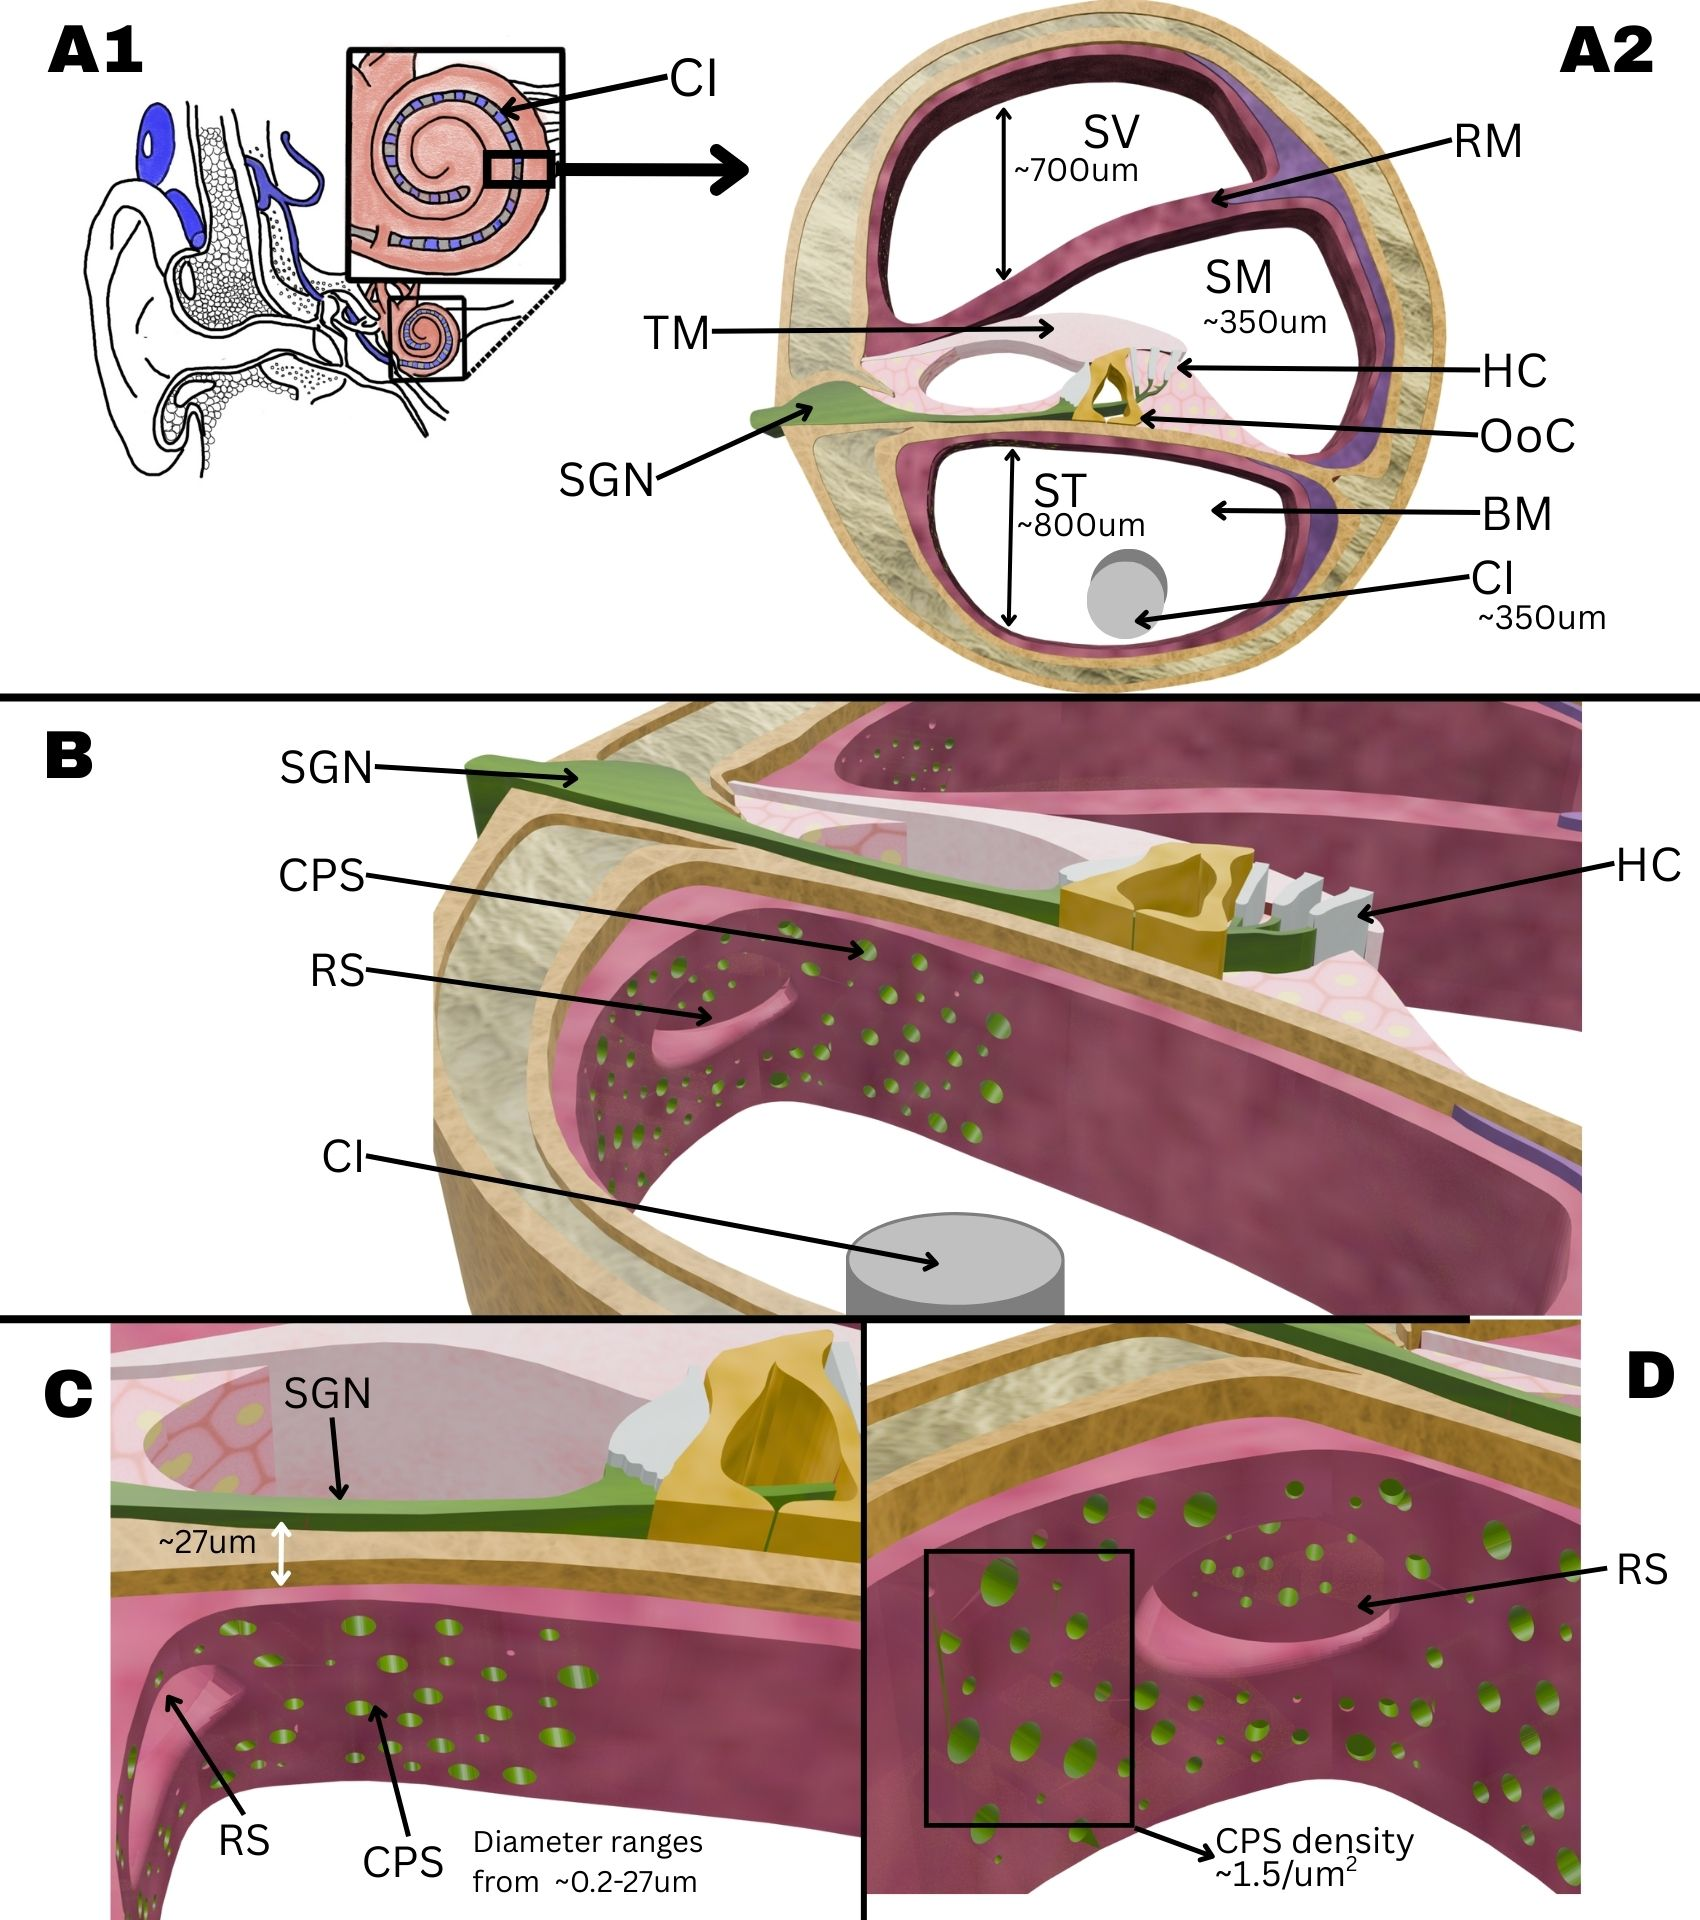
\includegraphics[width=0.89 \textwidth]{JNER_Submission/manuscript/figures/3DAnatomyPanel.jpg}
	\caption{Cochlear micro-anatomy and Canaliculi Perforantes of Schuknecht (CPS) in relation to a cochlear implant (CI). A1\textendash A2: Overview and basal-turn cross-section showing scala vestibuli (SV $\approx \SI{700}{\um}$), scala media (SM $\approx \SI{350}{\um}$) bounded by Reissner’s membrane (RM), organ of Corti (OoC) with Hensen’s cells (HC) and tectorial membrane (TM), basilar membrane (BM), and scala tympani (ST $\approx \SI{800}{\um}$). A CI ($\approx \SI{350}{\um}$) lies within ST adjacent to the osseous spiral lamina containing spiral ganglion neuron (SGN) processes. B: Oblique cut-away illustrating the field of CPS (green) along the laminar ridge (RS) between ST and the SGN region. C–D: Higher-magnification views of the CPS field; individual CPS openings span $\approx\SIrange{0.2}{27}{\um}$ in diameter, with local areal density $\approx$1.5 pores per \SI{1000}{\micro\meter\squared}, and the SGN layer thickness at this level is $\approx \SI{27}{\um}$ \cite{Schuknecht1959,schuknecht1963,lim1970,masuda1971,tanaka1973,shepherd2004}.}
	\label{fig:cochlea_overview}
\end{figure}
%%%%%%%%%%%%%%%%%%%%%%%%%%%%%
\subsection{Cochlear scalae in brief}  
Within the cochlea of the bony labyrinth, the perilymph-filled scala vestibuli (SV) and ST, spiral around the modiolus and are continuous at the helicotrema; between them lies the endolymph-filled scala media (SM) (i.e., the cochlear duct) of the membranous labyrinth (Fig. \ref{fig:cochlea_overview} A1 \& A2). Conventional cochlear implants occupy the ST (Fig. \ref{fig:cochlea_overview} A1), placing their contacts within millimeters\textemdash rarely microns\textemdash of SGNs embedded in Rosenthal's canal (dendrite) and modiolus (cell body) (Fig. \ref{fig:cochlea_overview} A2) \cite{Starovoyt2023_SciRep_CochlearMicrostructures,Micuda2024_Laryngoscope_SRPCI_ST}. Importantly, typical electrode-to-SGN distances are around $\SIrange{0.5}{1}{\mm}$ for modiolus-hugging arrays and up to SM $\approx \SIrange{1.5}{2}{\mm}$ for lateral wall placements \cite{Sharma2024_Laryngoscope_EMDApproach}. Even in the best-case scenario, a gap on the order of $10^{2}-10^{3}{\um}$ remains between the electrode and SGNs \cite{Sriperumbudur2024_SciRep_EfieldPorosity}. This physical separation has practical implications: it necessitates current spread through perilymph and bone to reach the SGNs, and it underlies why closer electrode positioning (e.g. perimodiolar designs) can reduce stimulation thresholds \cite{Kawano1998}. Furthermore, the distance can vary along the cochlea \textemdash apical electrodes often achieve the smallest gaps $\approx \SI{0.5}\mm$ or less) while mid-cochlear electrodes can be $\approx \SI{1}\mm$ or more away \cite{Long2014}. These quantitative insights, drawn from human studies, validate that CIs interface with the SGNs across a millimeter-scale gulf, rather than forming direct micron-level contact with the neurons. Finally, any natural pores linking the ST to the modiolus are therefore potential highways for drugs, trophic factors, or neurites seeking the electrode array in the ST \cite{Braga2023_JARO_OSLmicroCT,Starovoyt2023_SciRep_CochlearMicrostructures}.
.

\subsection{Scala Tympani Dimensions and Cochlear Implant Feasibility}
\subsubsection{Scala Tympani Anatomy in Humans}
\paragraph{Human [Homo Sapiens]}
As briefly mentioned in a previous section, the human ST is a large perilymph-filled canal that narrows from base to apex (Fig. \ref{fig:cochlea_overview} A1 \& A2). Near the basal turn (around the round window region), the ST cross-section is ovoid with a typical vertical height of $\approx \SIrange{1.2}{1.4}{\mm}$ and width slightly larger \cite{fujiwara2023morphometric}. This corresponds to a cross-sectional area of roughly $\SI{2.3}{\mm^{2}}$ at the base ($0^{\circ}$), which then diminishes to about $\SIrange{1.3}{1.4}{\mm^{2}}$ by $180^{\circ}$ (half a turn) into the cochlea \cite{fujiwara2023morphometric,Micuda2024_Laryngoscope_SRPCI_ST}. Beyond the basal turn ($\approx \SI{360}{\degree}$), the ST lumen becomes more of a flattened triangle in cross-section as it enters the middle and apical turns. The height drops below 1 mm in the upper turns, and the area continues tapering (often $< \SI {1}{\mm}^{2}$ near the apex). Thus, the basal ST can accommodate larger diameters, whereas the apical region is very small and slit-like. Notably, the ST width is consistently greater than its height at any given point \cite{hatsushika1990dimensions}, reflecting the elongated shape of the duct. The human cochlea is $\approx \SIrange{35}{36}{\mm}$ in uncoiled length (2.5\textendash2.7 turns) and the total ST volume is $\approx \SI{29}{\micro\liter}$ \cite{Liu2023FEA}.

\subsection{Canaliculi Perforantes of Schuknecht (CPS)}  
Schuknecht's original temporal bone study (1959) revealed hundreds of microscopic channels piercing the osseous spiral lamina (OSL) from the ST toward the modiolus \cite{Schuknecht1959}. Later histology and scanning electron microscopy confirmed that these \textit{canaliculi perforantes} concentrate along the modiolar plate, especially in the basal and middle turns \cite{schuknecht1963, Schuknecht1959,lim1970, masuda1971,sando1971, tanaka1973, tanaka1976}. The CPS are predominantly located on the ST surface of the OSL, in the lower (inferior) bony lamina that underlies the basilar membrane. They are especially numerous in the modiolar (medial) region of the OSL, adjacent to the modiolus where the SGNs are housed \cite{shepherd2004} (Fig. \ref{fig:cochlea_overview} B, C \& D). Human CPS lumina were measured from 0.2 to 27 $\mu$m against an OSL thickness that tapers from 26.8 $\mu$m basally to 8.4 $\mu$m apically with local areal density $\approx 1.5 pores per \SI{1000}{\micro\meter\squared}$ (Fig. \ref{fig:cochlea_overview} C) \cite{shepherd2004, Braga2023_JARO_OSLmicroCT}. These dimensions overlap both the caliber of regenerating SGN neurites and the 10\textendash30 $\mu$m diffusion length of neurotrophins such as Neurotrophin-3 (NT-3) or Brain-Derived Neurotrophic Factor (BDNF) in perilymph, making each pore a matched conduit for axonal ingress and trophic support \cite{Green2012}.

\subsection{Other modiolar communication routes}
Rask\textendash Andersen and colleagues identified additional trabecular “meshwork”–like apertures within the modiolar trabecular network—measuring up to 100 $\mu \mathrm{m}$ on the SV side and approximately 40 $\mu\mathrm{m}$ on the ST side—together with fenestrations along perivascular and perineural sheaths \cite{raskandersen2006}. Together with the CPS, these openings establish a porous continuum that contradicts the notion of an impervious modiolar wall, permitting pressure equilibration and macromolecular traffic between perilymph and the SGN somata \cite{raskandersen2006, shepherd2004}. Most recent fresh-frozen CECT reproduced these soft-tissue corridors \cite{Starovoyt2023_SciRep_CochlearMicrostructures}.

In addition, the same investigators described “larger modiolar vascular outlets”, namely larger bony openings (up to $\approx \SI{100}{\um}$) situated adjacent to the anterior and posterior spiral modiolar veins and arteries \cite{raskandersen2006, shepherd2004}. The likely role of these vascular outlets is to permit exchange between the perilymphatic space and perivascular compartments, thereby contributing to perilymph homeostasis and offering potential routes for drug delivery \cite{raskandersen2006, shepherd2004}.

Complementing these channels, “mesothelial cell–covered fenestrae” were defined as thin cellular sheets ($< \SI{3}{\um}$), lining the OSL and the modiolar surface, interspersed with micropores (up to $\approx \SI{40}{\um}$) on both the ST and SV sides \cite{raskandersen2006, shepherd2004}. Functionally, the mesothelial cell–covered fenestrae provide a semi-permeable lining over the bony channels, allowing diffusion of both small and large molecules while maintaining fluid compartmentalization; at the same time, by facilitating exchange between perilymph and perivascular/perineural spaces, they support perilymph homeostasis and represent potential conduits for local pharmacologic access \cite{raskandersen2006, shepherd2004}. Table \ref{tab:channels_dimensions} summarizes quantitative dimensions of perilymph \textendash modiolar passage channels in the basal turn of the human cochlea. 

%%%%%%%%%%%%%%%%%%%%%%%%%%%%%%%%%%%
%Table to summerize thease numbers
%%%%%%%%%%%%%%%%%%%%%%%%%%%%%%%%%%
\begin{table}[ht]
	\centering
	\caption{Quantitative dimensions of perilymph?modiolar passage channels in the basal turn of the human cochlea.}
	\label{tab:channels_dimensions}
	\begin{tabular}{lll}
		\toprule
		\textbf{Structure / Channel} & \textbf{Dimension (basal turn)} & \textbf{Source} \\
		\midrule
		Canaliculi Perforantes Schuknecht (CPS) & Mean diameter $5.2 \pm 4.9\ \mu$m (range 0.2\textendash23.0 $\mu$m)       & \cite{ShepherdColreavy2004} \\
		Osseous spiral lamina (OSL) thickness & $26.8 \pm 6.0\ \mu$m                                      & \cite{ShepherdColreavy2004} \\
		Density of canaliculi (pores per \SI{1000}{\micro\meter\squared})   & $1.05 \pm 1.03$ pores per \SI{1000}{\micro\meter\squared}                                  & \cite{ShepherdColreavy2004} \\
		Mesothelial cell sheet thickness    & $0.3$\textendash$3\ \mu$m                                            & \cite{raskandersen2006} \\
		Trabecular mesh fenestrae size    & Up to $\approx 40\ \mu$m (holes in modiolar wall)             & \cite{raskandersen2006} \\
		Modiolar vascular outlets           & Pores up to $\approx 100\ \mu$m                               & \cite{raskandersen2006} \\
		\bottomrule
	\end{tabular}

    \par\vspace{2pt}
\noindent\footnotesize\emph{Note.} CPS density values \cite{ShepherdColreavy2004} are based on 2D pore counts per unit area in histologic sections. Recent 3D micro‑CT of the osseous spiral lamina reports comparable pore‑size distributions and regional enrichment near the modiolar plate, consistent with a porous OSL relevant to perilymph–modiolus communication \cite{Braga2023_JARO_OSLmicroCT}. \normalsize

\end{table}

\subsection{Functional pathways and SGN connectivity through CPS}
The CPS form a network of microscopic pores through the OSL that directly links the fluid of the ST with the perimodiolar spaces in Rosenthal's canal \cite{raskandersen2006}. By puncturing the lower plate of the OSL\textemdash alongside gaps in its mesothelial lining\textemdash and opening into the retrocolumnar trabecular meshwork and perivascular channels of the modiolus, these tiny canals create a continuous perilymphatic pathway from the ST into the SGNs. As a result, the extracellular fluid bathing the SGN cell bodies is essentially the same perilymph that fills the ST, permitting free interchange of ions, nutrients, signaling molecules, and even therapeutic agents or pathogens between these compartments \cite{Starovoyt2023_SciRep_CochlearMicrostructures}.

Although the true nerve fiber bundles use larger foramina (habenula perforata and modiolar conduits) to enter and exit Rosenthal's canal, the canaliculi perforantes run alongside and between those fiber routes, serving as perineural and perivascular fluid conduits. Glueckert et al. found nerve fibers in BDNF-treated animals that progressed into CPS. These fibers reveal a myelin layer close to the OSL and within the bony canaliculi but with extreme swelling when entering the ST \cite{glueckert2008}. Li et al. also observed SGN neurites projecting across the OSL wall into the ST through the CPS \cite{Li2017}. Similar observations have been reported by others \cite{Staecker1996, Leake2008, Leake2011, Wise2011}.  These findings provide strong support that a future biohybrid CI could leverage the CPS to establish synaptic connections between human iPSC-derived SGNs and endogenous SGN dendrites within the OSL and Rosenthal’s canal—an essential step toward reducing the electrode–neuron gap.

\subsection{Distance between cochlear implant electrodes and spiral ganglion neurons in Rosenthal's canal}
Conventional CI electrode arrays reside in the ST and thus are separated from the SGNs in Rosenthal's canal by the bony modiolus. Multiple anatomical and imaging studies confirm that across patients and electrode positions, the distance between an electrode contact and the SGNs in Rosenthal's canal generally spans from a few hundred microns up to $\approx \SIrange{1}{2}{\mm}$ \cite{Davis2016}. A detailed CT scan study of perimodiolar arrays reported a total range of $\approx \SIrange{0.1}{1.8}{\mm}$ in electrode-to-modiolus separation \cite{Long2014, Sharma2024_Laryngoscope_EMDApproach}. Histological section measurements estimate that in the human basal turn, a lateral-wall electrode may be roughly $\approx$ 2 mm away from the SGNs (by radial distance). These data support the statement that CI contacts lie within millimeters, but rarely mere microns of the SGNs \cite{Schmidbauer2023}.

The electrode-to-SGN distance is not uniform along the cochlea; it varies with the cochlear turn and electrode position. Overall, the closest electrode-neuron proximities are achieved in the apical cochlea, with mid-cochlea generally the farthest on average, though patient-specific anatomy causes considerable variability (overall 0.1\textendash1.8 mm range in the cited study) \cite{Long2014}.

\subsection{The electrode-neuron gap does matter}
Kawano et al. (1998) performed detailed histopathologic exams of five human cochleae with CIs and measured the distance between each electrode band and the center of Rosenthal's canal \cite{Kawano1998}. They reported that these electrode-to-SGN distances were in the millimeter range, and importantly found a correlation between greater distance and higher electrical thresholds and comfort levels. In other words, electrodes that sat farther (several millimeters) from the SGNs required more current to evoke hearing, reinforcing that distance is a key factor. The same study noted that intracochlear fibrosis or new bone formation could increase the electrode-modiolus distance, sometimes pushing contacts farther than their design intends. Nadol and colleagues, in histopathologic surveys, likewise estimated distances on the order of 0.5\textendash 2 mm and observed that any translocation of an array out of ST (or trauma to the modiolus) can reduce SGN counts, further emphasizing that the electrode-neuron gap matters \cite{nadol1990,Nadol1989}. Computational models and anatomic maps further illustrate these distances. For example, a recent finite-element model by Sriperumbudur et al. (2024) examined electrical stimulation with a perimodiolar CI and assumed a ~0.3 mm gap between the electrode and modiolus as a typical design \cite{Sriperumbudur2024_SciRep_EfieldPorosity}. This value ($300{\um}$) was chosen to reflect a snug perimodiolar placement, yet it still highlights that even in simulation the contacts are not assumed to be touching the neurons (a 0.3 mm gap leaves space for the bony wall and perilymph) \cite{Sriperumbudur2024}. 

\subsection{Surgical implications for biohybrid CIs}  
Because CPS density peaks in the basal OSL, traumatic insertion or aggressive drilling in this region risks sealing the very pathways that a biohybrid implant aims to exploit \cite{shepherd2004, Starovoyt2023_SciRep_CochlearMicrostructures}.  Conversely, electrodes engineered with microfluidic ports or neurotrophin-releasing sleeves could harness these pores to establish steep radial gradients that attract transplanted or residual neurites toward the contacts.  Designing arrays that spare, rather than violate, the CPS therefore becomes as important as thread depth, pitch, or perimodiolar curl.  Leveraging these natural conduits should reduce reliance on bulk diffusion, localize therapy to the modiolus, and ultimately tighten the electrode-neuron interface \textemdash a prerequisite for the stem-cell and material strategies developed in the following sections. Future biohybrid CIs are expected to incorporate microfluidic drug delivery to steer regeneration locally within the cochlea \cite{Carnicer-Lombarte:2025aa}.

%%%%%%%%%%%%%%%%%%%%%%%%%%%%%%%%%%%%%%%%%%%%%%%%%%%%%%%%%%%%%%%%%%%
\section{Human stem-cell derived assembloids and hydrogel scaffolds for a living cochlear implant}\label{sec4}
%%%%%%%%%%%%%%%%%%%%%%%%%%%%%%%%%%%%%%%%%%%%%%%%%%%%%%%%%%%%%%%%%%%
Biohybrid CI concepts rely on living neural elements (i.e., hiPSC-derived stem cells) that can mature, respond to therapy, and form or re-form synapses with endogenous SGNs \cite{Nella2022NeurotrophinGradients}. In practice, this means (i) supplying the \emph{right cells} in the \emph{right microenvironment} and (ii) coupling them to the device through a mechanically and electrochemically compatible interface. In this section, we outline why three-dimensional (3D) stem-cell constructs \textemdash from simple \emph{spheroids} to more complex \emph{assembloids}\textemdash are preferred over dissociated cultures \cite{Pasca2022}. Recent inner‑ear organoid/assembloid work has sharpened these arguments, reporting improved SGN‑like phenotypes, synaptic specialization, and better translational relevance over 2D models \cite{Moore2025_CellStemCell, vanDerValk2023_CellRep, Zhang2024_NRR}.
We will also discuss how xeno-free hydrogels can provide a cochlea-ready niche that also supports localized delivery and chronic electrical interfacing \cite{Fakhr2024PeripheralNerve}.


\subsection{Why 3D?\textemdash from spheroids, organoids to assembloids}
Dissociated, two-dimensional SGN cultures show fragile survival and limited maturation \cite{Corrales2006}, whereas 3D environments provide a pro-survival, pro-maturation niche with improved neuritogenesis, synaptic puncta, and electrophysiological properties closer to native SGNs \cite{Zine2021StemCells,Sun2023CellProlif, koehler2013, Koehler2013Nature, koehler2017}. Newer human cochlear organoid protocols report high-fidelity morphology and sensory–neuronal patterning that better match in-vivo benchmarks \cite{Moore2025_CellStemCell}.

Spheroids (single-lineage aggregates) are easy to form and improve retention and trophic support after transplantation relative to single-cell suspensions \cite{Chang2020ActaBiomaterialia}. A more recent synthesis emphasizes 3D micro-environments for SGN survival, neurite extension, and myelination \cite{Zhang2024_NRR}. Inner-ear \emph{organoids} adds rudimentary cyto-architecture and hair-cell \textendash to \textendash SGN ribbon synapses \cite{Koehler2013Nature,koehler2017,Sun2023CellProlif}. 
See also recent reports detailing synaptic specialization and long‑term culture stability in inner‑ear organoids \cite{Moore2025_CellStemCell}. \emph{Assembloids} intentionally combine multiple, precisely chosen cell lineages to recreate elements of the SGN microenvironment \textemdash, for example SGNs with Schwann cells, satellite glia, and a microvascular compartment \textemdash, achieving myelination, robust trophic support, and more mature firing phenotypes than neuron-only constructs \cite{Xia2023StemCellReports,Oliveira2023FrontiersPN}. Satellite‑glia regulation of excitability in human sensory ganglia and myelin biology has also been updated in recent studies \cite{LeBlang2024_bioRxiv}. Where hair cells are not required for the intended biohybrid CI function, assembloids can omit them to reduce complexity while retaining essential SC/vascular support.

Most recently, four‑factor small‑molecule cocktail (GENtoniK; 1 $\mu$M each GSK2879552, EPZ‑5676, NMDA,and BayK8644) accelerated maturation of hPSC‑derived neurons within one week, increasing neurite length, synaptic puncta density, and spontaneous action‑potential firing while shifting transcriptomes toward postnatal, synaptic programs \cite{Hergenreder:2024aa}. The emerging small-molecule maturation regimens (e.g., 'GENtoniK') can further accelerate human neuron maturation in 3D systems; when used, these require pharmacological validation of synaptic readouts and careful dose scheduling to maintain viability and lineage identity \citep{Hergenreder2024NatBiotech}.

\subsection{Design of SGN assembloids: cell composition and roles}
A practical SGN assembloid includes four interacting cell types whose functions are complementary: (i) \textbf{SGNs} (afferent neurons, the principal excitable elements) \cite{matsuoka_2017}; (ii) \textbf{Schwann cells} (myelination distal to the habenula; metabolic and trophic support; debris clearance; immune orchestration) \citep{Oliveira2023FrontiersPN,Moss2024iScience}; (iii) \textbf{satellite glia} (ion and neurotransmitter homeostasis around somata) \cite{Meas2018}; and (iv) \textbf{fibroblast/perineurial cells} (ECM deposition and compartmental definition) \cite{Constantin2024}. 
Recent comparative analyses of inner‑ear cell models and peripheral‑nerve micro-environments inform these lineage selections \cite{vanDerValk2023_CellRep, Jiang2024_EBioMedicine}. We \emph{deliberately omit a vascular compartment} in the intraluminal setting because the ST–facing bony wall lacks a perfusable vessel bed; expecting engineered endothelial–host anastomosis at this interface is unlikely and could promote fibrovascular responses \cite{Wright2018}. The perineurial barrier and endoneurial microenvironment impose tight transport constraints and are not trivially re‑created at the ST bony wall \cite{Iwanaga2022_BiomedRes, Jiang2024_EBioMedicine}. Instead, one could use a \emph{diffusion‑first} design: compact (~\(\leq\) 300\,\(\mu\)m) 3D units embedded in a porous ECM so that oxygen and trophic diffusion distances remain within avascular limits while preserving alignment and myelination. Co‑culture with 3D microfluidic environment favors compact myelin formation around peripheral axons and higher‑amplitude, more phase‑locked firing, with evidence of ribbon synapses in innervated cochlear organoid systems \citep{Xia2023StemCellReports}. See also organoid/assembloid systems that report robust SGN‑like firing and synaptic markers \cite{Moore2025_CellStemCell}.

Placement against the OSL with fronts facing the CPS (Section~\ref{sec3}) allows device-driven radial gradients (e.g., BDNF/NT-3) to recruit neurites through microchannels toward the modiolus rather than relying on neovascularization of the ST wall.

\subsubsection{Why target \texorpdfstring{$<$ 200\,$\mu$m}{< 200 µm}? }
Avascular neural assembloids become diffusion‑limited for O$_2$ and trophic factors once characteristic path lengths exceed $\approx$ 100\textendash200\,\textmu m; beyond that, hypoxia and necrosis develop at the core unless there is active perfusion or large, interconnected pores \citep{Grimes2014SpheroidOxygen,Rouwkema2008Vascularization,MuellerKlieser1987Spheroids}. 
Recent organoid engineering reviews reiterate the $\approx$200 $\mu$µm oxygen/nutrient diffusion limit for avascular tissues \cite{Chen2024_NatRevBioeng}. Designing SGN assembloids as disks/ellipsoids with a smallest dimension $<$ 150–200\,$\mu$ m (i.e., diameter $<$ 200\,$\mu$m if roughly spherical) keeps the half‑thickness within known avascular transport limits while still allowing enough cells for myelination and spike generation by Schwann‑supported SGNs \citep{Oliveira2023FrontiersPN,Moss2024iScience}. A porous ECM further reduces effective diffusion distances (lower tortuosity) and improves factor retention, which is important when shaping radial BDNF/NT‑3 gradients from the device face toward CPS (Sec.~\ref{sec3}) \citep{SandovalCastellanos2020HeparinBDNF,Nella2022NeurotrophinGradients,Leake2013}. Practically, we set acceptance criteria as: (i) geometric half‑thickness $<$ 150–200\,\textmu m, (ii) live–dead and hypoxia reporter readouts without a necrotic core at 48\textendash 72\,h in static culture, and (iii) sustained phase‑locked firing with Schwann co‑culture (indicating adequate oxygenation and ionic homeostasis) \citep{Xia2023StemCellReports}.

\subsubsection{Porous ECM for SGN assembloids: why laminin, and what to pair it with?}
As we discussed in our previous section, because the ST wall provides no perfusable vessel bed, we do not include a vascular compartment in intraluminal SGN assembloids. Instead, viability and function should be secured by (i) keeping constructs $\leq$ 200\,\textmu m in their smallest dimension, (ii) embedding them in a porous, neurite‑permissive ECM, and (iii) driving \emph{radial} trophic gradients from the device face toward CPS mouths (Sec.~\ref{sec3}) \citep{Nella2022NeurotrophinGradients,Leake2013,Evans2009-cm,SandovalCastellanos2020HeparinBDNF}. 

\paragraph{Why laminin as the spine?} Laminins are the dominant basement‑membrane ligands for both SGNs and Schwann cells; they engage laminin‑binding integrins to promote neurite extension, Schwann alignment, and myelination \cite{Evans2007LamininFibronectin}. In peripheral nerve and basal lamina‐like matrices, laminin isoforms consistently bias outgrowth and support compact myelin, while reducing the need for non‑specific RGD cues that can recruit fibroblasts \citep{Evans2007LamininFibronectin,Vega1995LamininCollagenIV}. Recombinant human laminin‑511/521 (or laminin‑derived peptides [e.g., IKVAV and YIGSR]) provides a defined, xeno‑free backbone that is highly neuritogenic and compatible with GMP manufacturing \cite{Lu2014XenoFreeIPS}. “A more recent review highlights laminin‑511/521 as preferred xeno‑free matrices in clinical‑grade hPSC systems \cite{Ozawa2023_BiomaterTransl}.

\paragraph{Other Extracellular Matrices}
Collagen IV complements laminin to form a basement‑membrane–like network that SGNs and Schwann cells recognize; it stabilizes laminin and provides gentle scaffold strength without forcing high stiffness \citep{Yurchenco2011BasementMembranes,Yurchenco2009Laminins,Feltri2005LamininsSchwann}. 
Recent overviews of Schwann‑cell–ECM dynamics and peripheral‑nerve matrices support laminin‑biased, low‑stiffness blends for neurite guidance \cite{Jiang2024_EBioMedicine}. Collagen I, in contrast, forms fibrillar, typically stiffer gels that are broadly pro‑adhesive (RGD‑rich) and can favor fibroblast infiltration \citep{Shoulders2009CollagenStability,Hersel2003RGDReview,Frantz2010ECMGlance,Discher2005Stiffness}. In an intraluminal niche where fibrosis is undesirable, a laminin$+$collagen IV matrix can be more favorable; if collagen I is used at all, we could keep it dilute and blended with laminin (and/or hyaluronan) to keep the bulk modulus low and neurite‑friendly \citep{Bonnans2014ECMRemodel,Feltri2005LamininsSchwann}. Vitronectin and fibronectin\textemdash RGD‑rich proteins are excellent for hiPSC maintenance and general adhesion, but they are less specific for SGN/Schwann programs and can potentiate fibroblast attachment. Use them sparingly (e.g., as micro‑patterned adhesion islands for initial handling) or omit them in favor of laminin‑biased ligands (IKVAV, YIGSR) when the goal is long‑term neuronal alignment and myelination \citep{Evans2007LamininFibronectin}. 

\paragraph{Porosity and mechanics.}
To prevent core necrosis without perfusion, the ECM should match brain/nerve‐like moduli ($\approx$0.5–3~kPa) and incorporate \emph{intrinsic microporosity} to shorten diffusion paths and lower tortuosity \citep{Discher2005Stiffness,Budday2015BrainMech,Seidlits2010HALaminin}. 
Recent cryogel reviews and microporous‑hydrogel advances (granular/annealed‑particle) provide practical routes to cell‑scale porosity at neural‑range moduli \cite{Omidian2023_FrontBioengBiotech, Yang2023_SciAdv, Wang2025_FunctBiomat_MAP}. Practical routes include sacrificial gelatin/alginate microspheres or microfibers yielding interconnected 20–80\,\textmu m pores, cryogelation to form supermacroporous, highly permeable networks, and microporous‐annealed‐particle (MAP) gels assembled from microgels (“annealed microgels”) for cell‐scale porosity and rapid mass transport \citep{Bencherif2012Cryogels,Lozinsky2018CryogelsReview,Griffin2015MAP,Highley2016HAReview}. Hyaluronan‐rich blends further increase water content, reduce matrix friction, and support neurite outgrowth when combined with laminin cues \citep{Seidlits2010HALaminin,Highley2016HAReview}. Geometrically, keeping the smallest spheroid axis $\lesssim$150–200\,\textmu m (i.e., diameter $\leq$300\,\textmu m if roughly spherical) respects avascular diffusion limits for O$_2$ and macromolecular trophic factors \citep{Sykova2008Diffusion,Grimes2014SpheroidOxygen}, which should be verified empirically (live–dead/hypoxia reporters; physiology) in static culture.

\subsection{Hydrogel scaffolds as the SGN assembloid niche}
The clinical translation of a bio‑hybrid cochlear implant hinges on a three‑dimensional scaffold that is both \emph{xeno‑free}—to eliminate batch‑to‑batch variability, undefined growth factors, and potential zoonotic agents intrinsic to matrices such as Matrigel. Candidates should possess self-assembling peptides, which are short synthetic peptides that spontaneously organize into nanofibers and form 3D hydrogels used as ECM-mimicking scaffolds for future biohybrid CIs. Lastly, they should be acoustically transparent, so that surface‑acoustic‑wave (SAW) energy can couple efficiently to the embedded SGN assembloids for any manipulation (see Section~\ref{sec7} for detail) \cite{Aisenbrey2020,Kozlowski2021,Sebastian2023}. Microscale acoustofluidic manipulation within soft, highly hydrated gels has been demonstrated across multiple platforms \cite{Zhang2020_AcousticMicrofluidics} (contextual review). Several \textit{in vitro} studies show that hydrogels with low shear modulus and minimal internal friction transmit SAW with negligible attenuation, whereas stiff, highly cross‑linked networks behave as mechanical low‑pass filters \cite{Sebastian2023,Liao2008,Haruna2020}. Hydrogels are logical load‑bearing supports for any membrane‑mimetic interfacial layers on CI electrodes \cite{Carnicer-Lombarte:2025aa}.

\subsubsection{VitroGel\texorpdfstring{\textsuperscript{\textregistered}}{ (R)} NEURON} 
VitroGel\textsuperscript{\textregistered} NEURON is a fully synthetic, xeno-free polysaccharide hydrogel that gels at room temperature by ionic exchange (no thermal or chemical initiators) \cite{TheWell_GelationWorks,TheWell_NeuronPage}. Ready-to-use formulations show a storage modulus of \(\sim\)100–300~Pa (manufacturer rheometry), corresponding to a Young’s modulus of \(\sim\)0.3–0.9~kPa \citep{TheWell_ReadyToUseModulus}. The system is supplied with compatible peptide-functional VitroGels (RGD, IKVAV, YIGSR) to dial in neurite-permissive cues \citep{TheWell_RGD,TheWell_IKVAV,TheWell_YIGSR}. Its transparent, physically cross-linked network supports shear-thinning and self-recovery typical of ionic polysaccharide gels—useful for handling and for dissipating micro-strain—while maintaining imaging compatibility \citep{TheWell_NeuronPage,Karvinen2022SelfHealing,Nishimura2023SelfHealing}.
Note that independent peer‑reviewed characterization for neuron cultures remains limited, so we report the vendor’s rheology and kit specifications here \cite{TheWell_RGD,TheWell_IKVAV,TheWell_YIGSR,TheWell_NeuronPage, TheWell_ReadyToUseModulus, TheWell_GelationWorks}.


\subsubsection{PeptiGel\texorpdfstring{\textsuperscript{\textregistered}}{ (R)} Alpha 4 vs.\ Alpha 4 PLUS}

We also here focus on PeptiGel\textsuperscript{\textregistered} Alpha~4~PLUS as a default SAP scaffold near cochlear-implant electrodes because it preserves the soft Alpha~4 mechanical profile (vendor rheometry: $G'\!\sim$0.7–1.3 kPa) and net positive charge, while introducing fibronectin-mimetic RGD and collagen-mimetic GFOGER motifs to engage integrins that support neural adhesion \citep{MBG_Alpha4,MBG_Alpha4PLUS,Hersel2003RGDReview,Knight2000GFOGER}. By contrast, Alpha~4 lacks these built-in adhesion cues and is best framed as a platform for custom laminin-derived tethering (e.g., IKVAV/YIGSR) when SGN-specific guidance is desired \citep{Silva2004IKVAV,Evans2007LamininFibronectin}. The auditory literature consistently indicates that laminin-biased cues (full-length laminin or its peptide mimetics) promote SGN neurite extension and directional guidance more effectively than generic RGD alone \citep{Evans2007LamininFibronectin,Relvas2001IntegrinsNervous,Chen2014MicrogroovedLaminin}. In practice, either (i) Alpha~4~PLUS can be used “as supplied” when broad integrin engagement is desired at the device face, or (ii) Alpha~4 can be functionalized with laminin-derived sequences to bias SGN/Schwann programs in a more lineage-specific manner, keeping the bulk modulus in the neural range. Also see Table~\ref{tab:hydrogel-comprehensive} summarizes all six candidate animal-free hydrogels evaluated against these criteria.
%–––––––––––––––––––––––––––––––––––––––––––––––––––––––––––––––––––––––––––––
% Table III: Comprehensive comparison of animal-free hydrogels for Layer 3 niche
%–––––––––––––––––––––––––––––––––––––––––––––––––––––––––––––––––––––––––––––
\begin{table}[ht]
  \centering
  \scriptsize
  \caption{Comprehensive comparison of candidate animal-free hydrogels for the hiPSC-derived SGN assembloids niche}
  \label{tab:hydrogel-comprehensive}
  \setlength\tabcolsep{7pt}
  {\renewcommand{\arraystretch}{1.35}% ← add this line (tune 1.2–1.6 as needed)
  \begin{tabular}{@{} 
      >{\raggedright\arraybackslash}p{0.15\linewidth}
      >{\raggedright\arraybackslash}p{0.35\linewidth}
      >{\raggedright\arraybackslash}p{0.20\linewidth}
      >{\raggedright\arraybackslash}p{0.10\linewidth}
      >{\raggedright\arraybackslash}p{0.24\linewidth}
      @{}}
    \toprule
    \textbf{Hydrogel (supplier)} &
    \textbf{Composition \& salient features} &
    \textbf{Pore / mesh size} &
    \textbf{Young’s $E$ (kPa)} &
    \textbf{SAW suitability} \\ 
    \midrule

VitroGel\textsuperscript{\textregistered} NEURON  (TheWell Bioscience) &
    Fully synthetic, xeno-free polysaccharide network; shear-thinning; customizable peptides. &
    Nanoporous ($\approx$ 200\textendash500 nm pore size) &
    0.3\textendash 0.9 &
    \textbf{Excellent}: low acoustic attenuation; rapid recovery \\

PeptiGel\textsuperscript{\textregistered} $\alpha$4 PLUS 
    (Cell Guidance System) &
    Self-assembling $\beta$-sheet peptide; pre-functionalized with adhesive SAP (RGD and GFOGER) & $\approx$ 100 nm fibers &
    0.7\textendash 1.3 & Good: moderate attenuation; built-in adhesion motifs \\

PuraMatrix\textsuperscript{\textregistered} (Corning) &
    Ionic RADA16 peptide nanofibrils; $>$ 99 \% water; amphoteric surface. &
    50\textendash200 nm fibers &
    0.1–1 &
    Fair: very soft; prone to micro-collapse \\

RGD-alginate (NovaMatrix FMC) &
    $Ca^{2+}$-crosslinked alginate grafted with RGD; enzymatically degradable. &
    $<$ 5 nm mesh &
    3\textendash20 & Poor: rapid gelation; high stiffness blocks SAW \\

HyStem-HP (Sigma) &
    Thiolated HA + gelatin + PEGDA; heparin-binding; tunable gel time. &
    $\approx$ 17 nm mesh &
    0.3\textendash 2 & Acceptable: moderate damping; 5 min work-time \\

PEG-DA hydrogels (Academic) &
    Photocrosslinkable PEG network; inert unless RGD-modified. &
    5\textendash10 nm mesh &
    0.5\textendash20 &
    Mixed: high impedance unless low-crosslink/RGD added \\
    \bottomrule
  \end{tabular}
  }% end local arraystretch
\end{table}

In summary, a minimal design rule emerges: choose a \emph{xeno-free, soft (0.5\textendash3 kPa), peptide-adhesive} gel that can be injected and quickly recover, then decorate with ECM motifs (RGD/IKVAV/YIGSR) and gradients of neurotrophins (e.g., BDNF/NT-3) to bias neurite trajectories. In several cochlear and neural contexts, peptide-functionalized hydrogels attract SGN neurites and support long-term survival; in inner-ear models, nanofibrillar cellulose and related systems have been used to create a 3D niche with \emph{sustained} factor release \citep{Pancratov2017ColSurfB,Chang2020ActaBiomaterialia}.  hiPSC-derived SGN assembloids offer a controllable, multi-lineage route to a living CI interface, while modern, xeno-free hydrogels supply the compliant, bioactive niche and delivery vehicle those cells need. When combined with conductive and anti-fouling coatings, these materials can narrow the effective electrode-neuron distance and maintain implant performance while enabling regeneration-driven improvements over time.

%%%%%%%%%%%%%%%%%%
\section{Biomaterial interfaces for next-generation cochlear implants}\label{sec5}
%%%%%%%%%%%%%%%%%%%%
Biohybrid 'living' cochlear implants must balance three coupled demands: (i) efficient charge transfer at the metal-tissue boundary, (ii) mechanical and electrochemical compliance to match inner-ear tissues while maintaining stable stimulation and recording, and (iii) durable resistance to fibrosis, infection, and biofouling. A practical material stack proceeds from established noble-metal contacts to conductive polymer interlayers, then to conductive hydrogels and anti-fouling chemistries that enable regenerative and drug-delivery functions \cite{CarnicerLombarte2024AdvMat}.

\subsection{Platinum-Iridium (Pt-Ir): the clinical baseline}
Platinum-iridium (Pt-Ir) remains the workhorse for intracochlear electrodes due to corrosion resistance and long clinical track records. Chronic stimulation studies continue to refine safe operating windows and dissolution limits, and thin-film variants have been characterized electrochemically and in vivo \cite{Shepherd2020,Dalrymple2020, Vecchi2024}. Pt-Ir establishes a reliable, inert foundation but offers limited mechanical compliance and comparatively modest charge-injection capacity relative to newer coatings.

\subsection{Indium tin oxide (ITO) in living biohybrid interfaces.}
ITO is an optically transparent conductive oxide long used to make \emph{transparent} microelectrode arrays (MEAs) \cite{Weaver2022_JNE_TransparentMEA}, enabling simultaneous optical interrogation (e.g., imaging or optogenetic actuation) and electrical readout of living neural cultures \citep{Gross1985ITO,Weaver2022TransparentMEA,Kunori2015ITOEpidural}. For a biohybrid CI concept, that transparency can be leveraged during ex vivo assembly/testing of SGN assembloids on the array (morphology, Ca$^{2+}$ imaging) and, in optogenetic prototypes, to minimize photoelectric artefacts while preserving electrical access \citep{Cho2022TransparentImplants, Kunori2015ITOEpidural}. The main liabilities of ITO are (i) higher impedance/noise than classic neuroelectrode materials and (ii) brittleness on flexion; recent studies therefore use ITO primarily for \emph{transparent traces/windows} and add low‑impedance micro‑islands (PEDOT, IrOx, or ultrathin TiN) at the actual stimulation sites \citep{Ryynanen2019ALDTiN,Ryynanen2020IBAD}. Practically, this hybrid stack retains optical access for living tissue while restoring electrochemical performance to neuroprosthetic norms. Where neurite guidance is desired, ITO and over‑coats can be further functionalized with laminin‑biased cues (full‑length laminin or IKVAV/YIGSR peptides); in vivo work with laminin‑coated CI electrodes has shown enhanced neurite targeting and lower ABR thresholds, underscoring the value of laminin chemistry at the interface \citep{Bas2019LamininCI,Parys2022InnerEarTherapy}.

\subsection{Conductive polymers (CPs)}
Conductive polymers such as PEDOT:PSS and polypyrrole (PPy) lower impedance and increase charge injection capacity over bare Pt-Ir, improving the efficiency of neural interfaces \cite{Venkatraman2011-ql,Jow2023_APLBioeng_PEDOTPt}. PEDOT and PPy coatings can be patterned or covalently anchored to metals to enhance adhesion and water stability \cite{Kleber2017,Chhin2018,Chen2024_NatRevBioeng}. Beyond electrochemistry, CPs have served as drug/growth factor reservoirs at the cochlear interface; for example, PPy matrices loaded with NT-3 or BDNF promoted neurite outgrowth from auditory neurons in preclinical models \cite{Richardson2007,Richardson2009,Evans2009-cm}. Overall, CPs are a mature route to reduce impedance and introduce biomolecule functionality, though long-term cohesion and delamination under intracochlear micromotion remain design concerns \cite{li2025pedot} and it may be premature to fully transition from Pt-Ir at this stage for biohybrid CIs. 

\subsection{Conductive hydrogels (CHs)}
Conductive hydrogels (CH) combine soft, tissue-like mechanics with ionic/electronic transport, further reducing interfacial impedance while improving conformal contact with the modiolar wall \cite{Green2012}. In cochlear and related neural contexts, CH coatings improved electrochemical performance and chronic stability under stimulation \cite{Hassarati2014,Dalrymple2020,Hyakumura2021, Pandey2023_MRSC_CHReview}. Practical integration typically uses a thin CP ``tie'' layer (e.g., PEDOT) or surface roughening/priming to secure the hydrogel mechanically and chemically to the metal contact \cite{Kleber2017,Chhin2018}. Because the hydrogel phase can host cargos, CHs are attractive vehicles for anti-inflammatory agents and neurotrophins at the electrode--neuron interface \cite{Green2012,Hassarati2014}.

\subsection{Poly(\texorpdfstring{$\varepsilon$}{epsilon}-Caprolactone): Structural carriers and drug depots}
Poly($\varepsilon$-caprolactone) (PCL) is a semicrystalline, FDA-cleared aliphatic polyester whose low glass-transition temperature (-60C$^{\circ}$) confers exceptional flexibility at body temperature. In its electro-spun or supercritically-foamed forms, PCL attains porosities of 40–65 \% with inter-connected pores between 20 $\mu$m and 60 $\mu$m, dimensions large enough for neurite penetration yet small enough to maintain mechanical integrity. A bulk (tensile) modulus of 30\textendash 60 MPa places PCL two orders of magnitude below metal conductors while remaining rigid enough to carry the shear loads of round-window insertion. Hydrolytic degradation proceeds slowly (months–years) via ester-bond scission, yielding non-acidic $\varepsilon$-caproic acid that diffuses readily from the cochlea and minimizes pH excursions \cite{Chen2024_NatRevBioeng}. These attributes make PCL an ideal intermediate layer: (i) it buffers the soft hydrogel–metal interface; (ii) its macro-pores act as high-capacity reservoirs for PODS-encapsulated neurotrophins; and (iii) aligned nanofibers provide topographical cues that “funnel” SGN neurites toward the conductive contact pads \cite{Pandey2023_MRSC_CHReview}. Recent work by Ramirez et al. \cite{Ramirez2024} strengthens this rationale: electro-spun PCL mats with approximately 0.4 $\mu$m fibers ($\approx$40 \% porosity) retained an ultimate tensile strength of $\approx$0.5 MPa and a Young’s modulus of 19 MPa, values that sit comfortably inside our mechanical-buffer window. When over-coated with a 0.3–0.4\,$\mu$m fibrin layer, the scaffolds overcame PCL’s native hydrophobicity, doubled cell retention, and supported hiPSC-derived neural progenitor cells through full dopaminergic differentiation. Neurite extensions exceeded 100 $\mu$m, tyrosine-hydroxylase expression rose sharply, and spontaneous multi-unit firing was recorded on micro-electrode arrays, confirming functional maturation. Together with the slow-degrading, non-acidic chemistry of the backbone, these findings confirm that PCL—especially when combined with thin ECM coatings—provides a mechanically appropriate, neurotrophin-loadable, and electrophysiologically permissive scaffold for our biohybrid cochlear-implant design \cite{Li2007,Friend2011}.

\subsection{Anti-fouling and anti-inflammatory surface chemistries}
Surface chemistries that resist protein adsorption and cellular adhesion are increasingly being applied to CI carriers. Photografted zwitterionic hydrogels on clinical silicone carriers reduced the foreign-body response \textit{in vivo}, supporting their translational relevance for the cochlea \cite{Horne2023_ActaBiomater_ZwitterionCI}. In parallel, steroid-eluting arrays (dexamethasone) have advanced from preclinical to clinical evaluation, with studies reporting reduced impedances and inflammatory markers and ongoing assessments of hearing preservation and safety \cite{Kiefer2008Dexameth,Briggs2020,xu2018,Rahman2024,Toulemonde2021}. Together, anti-fouling and controlled-release strategies complement CP/CH stacks by modulating the host response over the critical peri-implant period.

\subsection{Sustained neurotrophin delivery and neurite guidance}
In the past decade, substantial progress has been made in delivering neurotrophic therapy to the inner ear \cite{StPeter2022}. Viral vector‑based gene delivery (AAV, Ad28) enables long-term localized expression of BDNF in supporting cells or SGNs. Modified promoters can minimize adverse effects from overexpression while maintaining therapeutic protein levels \cite{Leake2019, Mukherjee2022}. Hydrogel and nanoparticle depots—such as biodegradable hydrogels and nanoporous silica—provide controlled, sustained release of BDNF over weeks without requiring continuous infusion, improving protein stability and SGN preservation \cite{Wise2016, Yu2024, Zhang2024_JNanoBiotech_SGNProtect}. TrkB‑agonist mimetics, including small molecules like 7,8‑dihydroxyflavone or monoclonal antibodies, mimic BDNF effects while offering better pharmacokinetic stability and diffusion, bypassing issues related to large protein delivery with proven ability to promote SGN survival and synaptic repair ex vivo \cite{Szobota2019}.Cell-based coatings on electrode arrays using BDNF-secreting cells offer localized, on-site neurotrophic support, preserving SGNs and enhancing neurite regrowth in animal models \cite{Scheper2019}. Together, these strategies provide spatiotemporal control of BDNF delivery, balancing efficacy with safety for clinical translation.

\subsubsection{The Polyhedrin Delivery System (PODS\texorpdfstring{\textsuperscript{\textregistered}}{(R)})}
PODS\textsuperscript{\textregistered}–BDNF consists of BDNF co‑crystallized within a polyhedrin protein lattice to form stable, micron‑scale crystals \cite{Ikeda2006,Coulibaly2007,Coulibaly2009,Mori2007,Tanaka2007,Ijiri2009}. These depots resist dissolution and instead release BDNF as the lattice undergoes slow, local proteolysis, generating sustained, quasi–zero‑order release over weeks—an attractive counterpoint to the minute‑scale systemic half‑life of soluble BDNF (plasma $\sim$110\,min; CSF $\sim$60\,min) \cite{Mori2007,Poduslo1996,Sakane1997,Soderquist2009}. In cochlear‑relevant models, a longitudinal ``neurotrophic strip'' or gradient along the array is feasible using PODS embedded in sleeves/coatings, continuously bathing nearby SGNs \cite{Nella2022NeurotrophinGradients,Chang2020StemCellNiche}. Manufacturer stability data further indicate long‑term preservation of bioactivity within the crystalline state (e.g., $\sim$70\% activity at 6\,months at 37\textsuperscript{$\circ$}C) \cite{CellGS_PODS}.

Compared with alternatives, PODS targets the core delivery problems without introducing living cells or gene expression: AAV‑BDNF can achieve longevity but is hard to confine and overexpression can be maladaptive in normal cochleae \cite{Lee2016}; hydrogel or thin‑film depots often show early burst and taper within days–weeks \cite{Zimmermann2000}; nanoparticles/microspheres extend release but commonly retain an initial burst and incomplete elution \cite{Schmidt2018}; small‑molecule TrkB agonists diffuse well but have short half‑lives and have underperformed BDNF in preserving SGNs and function \cite{vink2022,heuer2021}; and encapsulated cell therapies add surgical and safety complexity with benefit limited to the implant period \cite{Pettingill2011}. By contrast, PODS–BDNF integrates directly with polymer/hydrogel carriers (e.g., PCL sleeves, conductive hydrogels) without loss of activity, maintains mechanical integrity of the composite, and supports device‑aligned gradients to recruit and sustain neurites at the interface \cite{Nella2022NeurotrophinGradients,Chang2020}.

\section{Surface Modifications to Enhance Neuron--Electrode Interactions}\label{sec6}
\
A persistent barrier to CI performance is the sub‑mm–to–mm electrode–SGN separation, which increases current spread and degrades channel selectivity. In a biohybrid CI, surface engineering can (i) lower the electrochemical barrier at the interface, (ii) physically guide neurites toward contacts, and (iii) suppress early protein fouling and chronic inflammation that would otherwise raise impedance and reduce neural proximity. Below are four complementary approaches and design considerations for integrating them into a regeneration‑supportive interface.

\subsection{Approach 1: Microstructured electrode surfaces}
Microscale topography biases SGN neurite alignment and expands the effective “capture radius” of contacts. Repeating ridge–groove patterns (periods $\sim$5–20\,\textmu m; depths $\sim$1–5\,\textmu m) increase alignment and turning fidelity via growth‑cone mechanosensation \cite{Wang2013,Chen2014}. In vivo, microgrooved CI electrodes show the expected trade‑off: better neurite guidance and stability versus insertion risk if features are sharp or too tall \cite{Lee2019}. Practical guidance: keep features shallow/rounded, embed them under a compliant coating, and co‑present permissive ECM ligands (e.g., laminin stripes) to amplify guidance without adding stiffness discontinuities \cite{Evans2007LamininFibronectin,Vega1995LamininCollagenIV}.

\subsection{Approach 2: Conductive and electroactive coatings}
Roughened noble metals and electroactive polymers reduce interfacial impedance and raise charge‑injection capacity. PEDOT and polypyrrole (PPy)—including PEDOT–hydrogel interpenetrating networks—produce large, stable impedance reductions and improved charge transfer under chronic stimulation \cite{Venkatraman2011-ql,Goding2017,Dalrymple2020,ABIDIAN20081273}. Biofunctionalization (e.g., RGD/peptide‑modified PEDOT; drug‑loaded PPy) supports adhesion and controlled factor release directly from the surface \cite{Chikar2012,Richardson2007,Richardson2009}. For a biohybrid stack, a thin PEDOT (stability) over PPy (loading) beneath a soft, conductive hydrogel matches tissue modulus while preserving low impedance and volume for trophic depots (Section~\ref{sec5}). Key checks: coating adhesion under accelerated aging, safe charge density in perilymph‑like saline, and retention of low noise after sterilization \cite{Venkatraman2011-ql,Dalrymple2020,Green2012}.

\subsection{Approach 3: Antimicrobial and pro‑healing interfaces}
Early bacterial colonization and the foreign‑body response jeopardize chronic function. Polydopamine (PDA) is a versatile primer that improves adhesion and can present bioactive peptides; on silicone CI carriers, PDA–peptide films increase cell adhesion and viability \cite{Schendzielorz2017}. Zwitterionic chemistries (e.g., sulfobetaines) grafted or deposited onto CI materials markedly reduce nonspecific protein adsorption and leukocyte adhesion, lowering inflammation and stabilizing the electrode–tissue interface \cite{Horne2023_ActaBiomater_ZwitterionCI,Chen2023_MTBio_ZwitterionCI}. Antioxidant/antibiofilm polysiloxanes (e.g., N‑acetyl‑L‑cysteine‑functional siloxanes) add broad antibiofilm activity while preserving elastomer stability \cite{Cozma2021-jb}. In layered designs, place these chemistries at the tissue‑facing surface while leaving underlying electroactive layers to handle charge transfer.

\subsection{Approach 4: Anti‑fouling and anti‑biofilm surface chemistry}
Hydration‑rich, charge‑balanced surfaces (zwitterions; hydrophilic brushes) resist the protein conditioning film that seeds fibroblast/macrophage recruitment and biofilms. Zwitterion‑modified CI materials show substantial reductions in postoperative infection and inflammatory adhesion, with preservation of low impedances versus unmodified controls \cite{Chen2023_MTBio_ZwitterionCI,Horne2023_ActaBiomater_ZwitterionCI}. Where antimicrobial action is required (e.g., revisions or high‑risk cases), choose chemistries with sustained bactericidal activity but low neurotoxicity; NAC‑functional polysiloxanes are compatible with elastomeric carriers \cite{Cozma2021-jb}. Validate (i) stability under electrical pulsing, (ii) sterilization compatibility, and (iii) retention of anti‑fouling function after insertion testing. Taken together, these surface modifications provide a practical route to shrink the functional electrode–neuron gap and stabilize the interface over time—both prerequisites for any biohybrid CI aiming to recover finer spectral resolution.

%%%%%%%%%%%%%%%%%%%%%%%%%%%%%%%%%%%%%%%%%%%%%%%%%%%%%%%%%%%%%%%%%%%%%%%%%%
\section{Surface-Acoustic-Wave (SAW) Acoustofluidics for the Biohybrid CI}\label{sec7}
%%%%%%%%%%%%%%%%%%%%%%%%%%%%%%%%%%%%%%%%%%%%%%%%%%%%%%%%%%%%%%%%%%%%%%%%%
\subsection{Fundamentals of SAW acoustofluidics}
Surface acoustic waves (SAWs) are Rayleigh‑type elastic waves that propagate along a piezoelectric surface with nanometre amplitudes and evanesce over roughly one acoustic wavelength into the substrate, thereby concentrating energy near the solid–liquid interface \cite{Friend2011,Yeo2014_SAWmicrofluidics}. When a SAW encounters a liquid, part of its energy radiates into the fluid at the Rayleigh angle, driving steady microflows (\emph{acoustic streaming}) and exerting acoustic radiation forces on suspended objects—two effects that underpin pumping, mixing, trapping, and patterning without contact \cite{Ding2013,Gedge2012_SAW, Friend2011,Yeo2014_SAWmicrofluidics}. Recent field‑level reviews also consolidate these principles for biofabrication and precision biomanipulation, underscoring SAW’s non‑contact, label‑free control of cells and tissues \cite{Wu2024_MicroNano,Rufo2022_NatCommun}.

\subsubsection{Key parameters and symbols.}
An interdigitated transducer (IDT)—interleaved metal fingers on a piezoelectric film or crystal—launches a SAW when driven at radiofrequency (RF). The wave frequency \(f\) (Hz), wavelength \(\lambda\) (m), and surface‑wave speed \(v\) (m\,s\(^{-1}\)) satisfy
\[
f \;=\; \frac{v}{\lambda}
\]
For a given substrate, \(v\) is the Rayleigh wave speed (typically a few km\,s\(^{-1}\)); smaller IDT finger pitch \(\Rightarrow\) shorter \(\lambda\) \(\Rightarrow\) higher \(f\) \cite{Friend2011,Yeo2014_SAWmicrofluidics, Bruus2015_Governing_Equations}. In SAW microfluidics, \(f\!\sim\!10\text{–}150\)~MHz (\(\lambda\!\sim\!20\text{–}400~\text{\textmu m}\)) provides body‑force densities suitable for single cells, spheroids, and organoids/assembloids \cite{Shilton2008_NanoDisp,Gedge2012_SAW}. Device‑integrated acoustic tweezers and membrane‑guided SAW actuators reported recently expand placement fidelity while maintaining microfluidic compatibility \cite{Vachon2023_LabChip,Yang2022_SteAST}. The electromechanical coupling coefficient \(K^2\) (dimensionless, often quoted in \%) measures how efficiently electrical energy is converted to acoustic energy; high‑\(K^2\) substrates (e.g., 128$^{\circ}$ YX–LiNbO\(_3\) with \(K^2\!\approx\!5\%\)) enable stronger waves for the same drive than thin‑film AlN/ZnO stacks \cite{Campbell1998,Yeo2014_SAWmicrofluidics}.

\paragraph{SAW–liquid coupling and the Rayleigh angle.}
Because the SAW phase velocity \(v\) in the solid exceeds the sound speed \(c_f\) in the fluid, the leaky wave radiates into the liquid at an angle \(\theta_R\) given approximately by Snell’s law,
\[
\sin \theta_R \;\approx\; \frac{c_f}{v},
\]
so for water (\(c_f\!\approx\!1500\)~m\,s\(^{-1}\)) on LiNbO\(_3\) (\(v\!\sim\!4000\)~m\,s\(^{-1}\)), \(\theta_R\!\approx\!22^{\circ}\) \cite{Friend2011,Ding2013}. The oscillatory viscous boundary layer thickness near the interface is
\[
\delta \;=\; \sqrt{\frac{2\nu}{\omega}},
\]
with kinematic viscosity \(\nu\) and angular frequency \(\omega=2\pi f\). For water, \(\delta\) is tens of nanometres at 10–100~MHz, which explains why streaming is generated efficiently even for nanometre SAW amplitudes \cite{Friend2011,Yeo2014_SAWmicrofluidics}. Printed and thin‑film SAW platforms (e.g., aerosol‑jet printed IDTs on flexible substrates) now realize these coupling rules in mechanically conformal formats \cite{Rich2024_MicroNano}.

\paragraph{Forces and flows (what moves the fluid and cells).}
Acoustic radiation force arises from gradients in acoustic energy density; for a small sphere (radius \(a\) \(\ll\) \(\lambda\)), the time‑averaged force can be written \( \mathbf{F}_{\mathrm{rad}} = -\nabla U \), where \(U\) is the Gor’kov potential that depends on pressure/velocity fields and on particle–fluid contrast factors (compressibility and density) \cite{Friend2011,Gedge2012_SAW}. This force scales with \(a^{3}\) and the square of acoustic amplitude, enabling selective trapping and patterning in standing‑wave fields (sSAW). Streaming is a second‑order (time‑averaged) flow generated by viscous rectification of the oscillatory motion near boundaries; characteristic streaming velocities scale with the square of the acoustic amplitude and increase with frequency until limited by viscous dissipation \cite{Ding2013,Friend2011}. In practice, traveling SAWs (tSAW) are used for pumping/mixing/transport via streaming, whereas sSAWs provide stable pressure nodes/antinodes for positioning cells and spheroids with micron‑scale precision \cite{Gedge2012_SAW,rufo2022}.

\paragraph{Operating bands and sensing.}
At ultra‑high frequencies (UHF–SAW; \(\sim\)300~MHz–3~GHz), \(\lambda\) becomes a few micrometres and the penetration depth into the substrate/fluid shrinks to sub‑micrometre, tightening energy confinement. The increased mass‑loading sensitivity of UHF resonators makes them attractive for label‑free biosensing of proteins, vesicles, or changes in viscoelastic properties at the surface \cite{Agostini2021_UHFSAW}. These regimes remain compatible with thin, flexible device stacks required in the inner ear \cite{Campbell1998}. At UHF (hundreds of MHz to GHz), SAW resonators attain high mass‑loading sensitivity that has been leveraged in recent biosensor implementations and surveys \cite{Wang2023_Sensors_SAWBiosensors}.

\subsection{Biohybrid CI implant constraints}
A SAW‑enabled biohybrid CI must meet neural‑implant design constraints: (i) \textit{Form factor}—IDTs and any microchambers must be ultra‑thin and conformal to the scala tympani; (ii) \textit{Power/thermal budget}—RF actuation must remain within tight wireless‑power and temperature limits; (iii) \textit{Biocompatibility/sterility}—piezoelectric films, metallization and adhesives must resist fouling/encapsulation in perilymph; and (iv) \textit{Mechanical compliance}—flexible stacks must tolerate micromotion without delamination or fatigue \cite{Campbell1998,Ding2013,Mandal2022,Friend2011,Yeo2014_SAWmicrofluidics,Gedge2012_SAW,TrolierMcKinstry2004_PiezoMEMS,Dagdeviren2014_ConformalPiezo,Cogan2008_NeuralElectrodes,Merrill2005_Waveforms,Sewell2009,ISO14708-7:2016_CI,ISO10993-1_2018_Biocompatibility,Agostini2021_UHFSAW}. Printed/flexible SAW embodiments reduce thickness and improve conformability—attributes directly relevant to intracochlear deployment \cite{Rich2024_MicroNano}.

\subsection{Handling and delivery of 3D SGN aggregates}
SAW fields can levitate, trap, translate, and pattern multicellular spheroids (20–300\,\textmu m) without contact, preserving viability and differentiation capacity \cite{rufo2022}. Contemporary ‘acoustic tweezers’ surveys detail multi‑spheroid assembly, rotation, and fusion with cell‑safe doses \cite{Wu2024_MicroNano}. Phase‑controlled (``digital'') acoustofluidic devices place trapping nodes at will to immobilize and arrange multiple spheroids/organoids, enabling bottom‑up assembly of tissue‑like architectures \cite{Cai2020_Biofabrication}. Broad reviews concur that SAW and related acoustofluidics are reliable for forming, patterning, and fusing spheroids/organoids for tissue engineering—capabilities directly applicable to positioning iPSC‑derived SGN spheroids and glial/fibroblast co‑aggregates near CI electrodes (see Section~\ref{sec4}) \cite{Wu2022_EngRegen,Wu2024_MicroNano,Zhang2020_AcousticMicrofluidics,Gedge2012_SAW}.

\subsection{Acoustic detachment and harvesting}
Traveling SAWs detach adherent cells and harvest intact spheroids gently and efficiently. Kurashina \emph{et~al.} reported $>\!95\%$ detachment of adherent sheets at 19.4~MHz (2~W\,cm$^{-2}$, 20\,s) with $>\!98\%$ viability and preserved focal adhesions \cite{Kurashina2019}; a follow‑up achieved $\sim$10\,$\times$ higher yield of intact spheroids versus enzymatic methods \cite{kurihara2022}. Intermittent tSAWs can thus lift iPSC‑derived SGN spheroids and guide them onto a device‑side hydrogel without chemical dissociation.

\subsection{Spheroid placement and patterning}
Counter‑propagating SAWs create pressure nodes/antinodes for micron‑scale positioning. Ladder IDT arrays enable 1D alignment; orthogonal pairs provide grid‑like arrangements that can be oriented to steer neurite outgrowth toward contacts. Closed‑loop placement is feasible by combining sSAW fields with real‑time imaging/feedback \cite{rufo2022,Gedge2012_SAW,Cai2020_Biofabrication, Gedge2015_Theory_of_Surface_Acoustic_Wave_Device}. Examples include sSAW/eSAW fields that position single cells or aggregates in grids and lattices with closed‑loop optical feedback \cite{Yang2022_SteAST,Wu2024_MicroNano}.

\subsection{Microfluidic gradients and neurotrophic delivery}
SAW‑assisted streaming provides pump‑ and mixer‑free control of local flows, enabling stable, tunable biochemical gradients for guidance and dosing \cite{Friend2011,Ding2013,Zhang2020_AcousticMicrofluidics}. On‑chip BDNF gradients reproducibly bias axon turning toward higher concentrations, validating controlled chemotaxis in vitro \cite{Huang2014_BDNF}. In cochlear interfaces, neurotrophins (BDNF/NT‑3) promote spiral ganglion neurite outgrowth toward electrodes and may help close the electrode–neuron gap \cite{Schmidbauer2023}. Translationally, an implantable intracochlear microfluidic device has already demonstrated safe, metered drug infusion into the scala tympani in vivo \cite{Sewell2009}, and SAW streaming could, in principle, replace reciprocating pumps to refresh micro-environments and superimpose \emph{spatio-temporally controlled} gradients from device‑side reservoirs \cite{Friend2011,Ding2013}. Reviews from 2022–2024 summarize acoustically driven pumping/mixing routes to spatio-temporally reconfigurable gradients suitable for chemotaxis assays and on‑chip dosing. \cite{Rufo2022_NatCommun,Wu2024_MicroNano}.

\subsection{Open questions and benchmarks.}
Key unknowns include: (i) stability of SAW‑generated gradients in perilymph; (ii) viability/phenotype of human SGN assembloids after repeated SAW exposure; (iii) long‑term drift of SAW device characteristics under chronic implantation; and (iv) whether UHF‑SAW sensing attains the dynamic range to track cochlear‑relevant neurotrophin (i.e., BDNF) levels in vivo \cite{rufo2022,Agostini2021_UHFSAW}. Resolving these will determine whether SAW modules become enabling components of biohybrid CIs or remain primarily ex vivo assembly tools.

%%%%%%%%%%%%%%%%%%%%%%%%%%%%%%%%%%%%%%%%%%%%%%%%%%%%%%%%%
\section{Conclusions and translational outlook}\label{sec8}
%%%%%%%%%%%%%%%%%%%%%%%%%%%%%%%%%%%%%%%%%%%%%%%%%%%%%%%%%


\noindent
Contemporary cochlear implants (CIs) restore audibility for hundreds of thousands of people, yet performance plateaus persist because the electrode–neuron separation blunts spatial selectivity and temporal fidelity \cite{wilson2008,wilson2014,Vecchi2024}. This review has synthesized convergent lines of evidence—anatomical, materials, cellular, and microfluidic/acoustic—that together outline a credible path toward \emph{biohybrid} interfaces: devices that co‑integrate with host or grafted neural elements, present targeted biochemical and mechanical cues, and maintain low‑impedance, stable electrochemistry over long durations \cite{CarnicerLombarte2024AdvMat,Green2012,Goding2017,Dalrymple2020}.

\paragraph{What is sufficiently established.}
First, classical and modern inner‑ear anatomy supports the existence of micron‑scale pathways in the modiolar region that can be leveraged for highly local delivery and guidance, rather than relying on bulk diffusion through perilymph \cite{raskandersen2006,lim1970,SaltPlontke2009,Leake2013}. Second, interface engineering has matured to the point where low‑impedance, tissue‑like coatings (conductive polymers and conductive hydrogels) can be paired with anti‑fouling chemistries without sacrificing charge injection or stability under clinically relevant duty cycles \cite{Green2012,Goding2017,Dalrymple2020,Horne2023}. Third, a broad preclinical literature shows that neurotrophic and related cues can bias spiral ganglion neurites, preserve somata, and improve interface‑level physiology when dosing is appropriately bounded in space and time \cite{Scheper2019,Chang2020,Kempfle2021,StPeter2022}. Finally, surface‑acoustic‑wave (SAW) acoustofluidics offers a contactless toolbox for microscale transport, mixing, and label‑free sensing that is inherently compatible with tiny volumes and soft, living constructs \cite{Friend2011,Ding2013,Agostini2021_UHFSAW}.

\paragraph{What must still be shown.}
Translation will hinge on quantitatively linking \emph{interface‑level} improvements to perceptual benefit while staying within the familiar surgical and safety envelopes for CIs. Concretely, reproducible gains in ECAP/eABR thresholds, spread‑of‑excitation, and channel independence should be demonstrated in vivo using clinic‑style pipelines \cite{Micco2006,Rebscher2008,wilson2008,wilson2014}. Inner‑ear transport constraints—mixing, longitudinal spread, and residence times—must be characterized at the scales that matter for guidance, with model credibility documented per current in‑silico guidance \cite{SaltPlontke2009,Leake2013,USFDA2021InSilico,ASMEVV40_2018}. On the materials side, long‑duration stability under intracochlear micromotion and stimulation remains the rate‑limiting evidence, particularly for multilayer stacks that combine electroactive coatings, soft gels, and antifouling/antimicrobial chemistries \cite{Dalrymple2020,Horne2023}.

\paragraph{Guardrails for safe progress.}
The likely regulatory framing is a \emph{combination product} (active implant plus drug/biologic), which implies a risk‑managed preclinical package spanning biocompatibility, chemical characterization, toxicology, leachables, dose–response, and chronic safety, alongside active‑implantable and CI‑specific standards \cite{ISO10993-1_2018_Biocompatibility,ISO14708-7:2016_CI}. Electrical dosing should remain within established charge‑density and waveform boundaries for neural tissue \cite{Merrill2005_Waveforms,Cogan2008_NeuralElectrodes}. Where computational models inform dose or safety margins, they should be paired with verification, validation, and uncertainty quantification, and cross‑checked against benchtop and \emph{in vivo} readouts \cite{USFDA2021InSilico,ASMEVV40_2018}.

\paragraph{A pragmatic outlook.}
Near‑term work across the field will be most impactful if it (i) anchors local delivery and guidance to anatomy that is demonstrably present in intended candidate populations \cite{raskandersen2006,lim1970}; (ii) standardizes interface‑level metrics (ECAP/eABR, spread‑of‑excitation) and transport characterizations to enable reproducible comparisons across platforms \cite{Micco2006,Rebscher2008}; and (iii) treats manufacturability and sterilization compatibility as first‑order design constraints, not afterthoughts \cite{Dalrymple2020,Horne2023}. Pre‑competitive datasets—microanatomy maps, material parameter sets for perilymphic environments, and benchmark modeling geometries—would accelerate this trajectory while keeping intellectual property with specific device embodiments.

\paragraph{Closing statement.}
If future studies can deliver an \emph{anatomy‑plus‑function} dossier—verified local access and dose control in the relevant modiolar microenvironment; durable, low‑impedance materials that co‑exist with targeted biochemical and mechanical cues; and robust, clinically interpretable gains at the interface—then biohybrid cochlear implants become plausible candidates for carefully bounded first‑in‑human evaluation. The destination is not a single recipe but a design space in which living and electronic components co‑evolve to close the electrode–neuron gap while respecting the clinical realities of cochlear implantation \cite{Vecchi2024, CarnicerLombarte2024AdvMat,wilson2008,wilson2014}.


\bibliography{bib}% common bib file
%% if required, the content of .bbl file can be included here once bbl is generated
%%\input sn-article.bbl
\end{document}
